\setLTR
\begin{lstlisting}
goto L5
L3: Stmt1
	goto L2
	goto L5
L1: Stmt2
L5: Stmt3
	goto L3
	goto L5
	goto L2
L4: Stmt4
	goto L1
	goto L4
L2: Stmt5
\end{lstlisting}
\setRTL

\qquad\qquad\qquad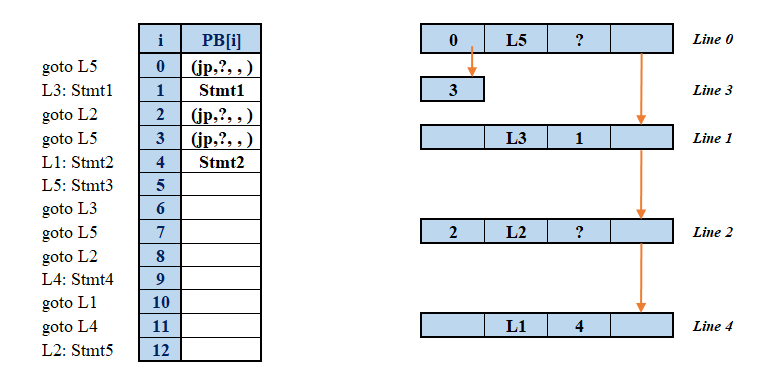
\includegraphics[width=0.7\linewidth]{figs/51.png} 

\qquad\qquad\qquad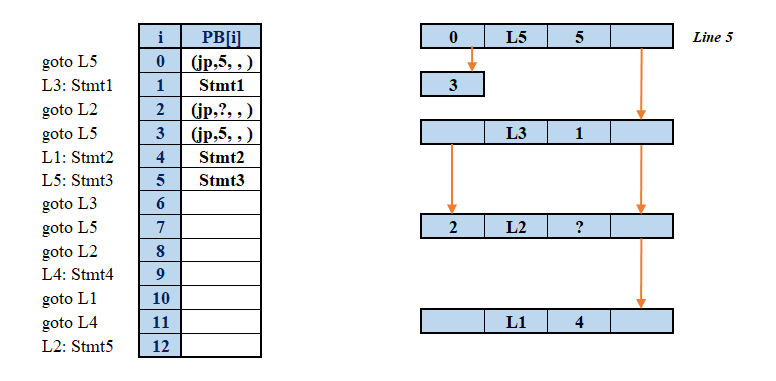
\includegraphics[width=0.7\linewidth]{figs/52.png} 

\qquad\qquad\qquad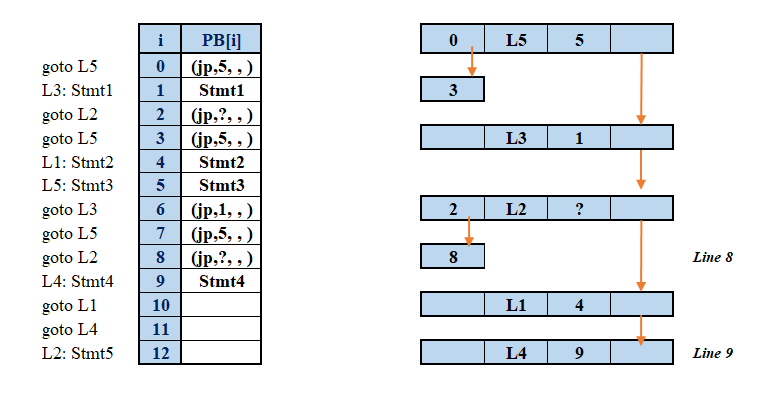
\includegraphics[width=0.7\linewidth]{figs/53.png} 

\qquad\qquad\qquad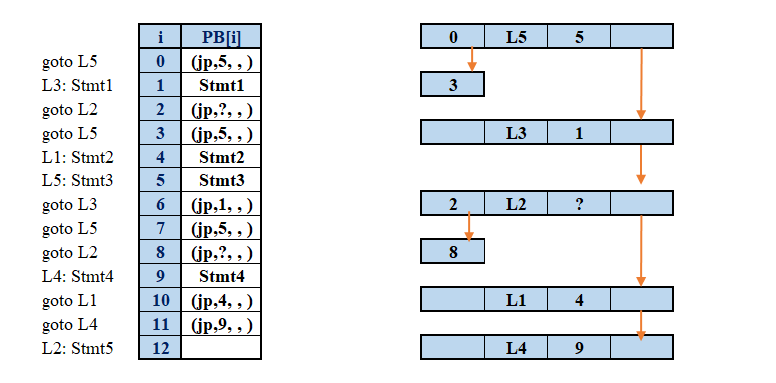
\includegraphics[width=0.7\linewidth]{figs/54.png} 

\qquad\qquad\qquad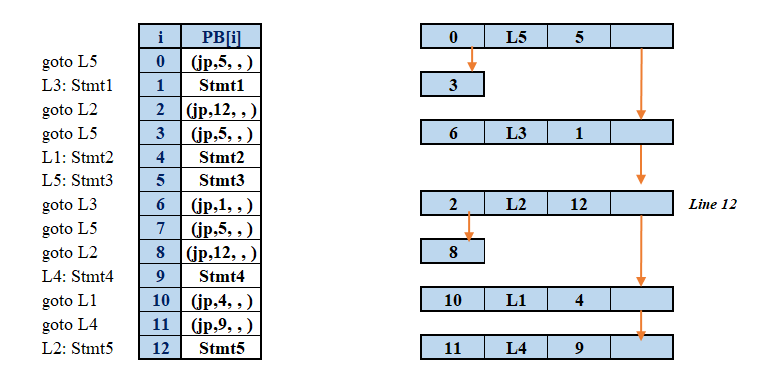
\includegraphics[width=0.7\linewidth]{figs/55.png}


\begin{itemize}
	\item 
	اگر پرش به لیبلی داشته باشیم که آدرس آن هنوز مشخص نیست، یک خانه خالی داخل 
	$Liked \ List$
	ایجاد می‌کنیم.
	\item 
	در هر مرحله از رسم نمودار، دستوراتی را نشان می‌دهیم که به هم ربطی ندارند و روی هم تاثیر نمیگذارند.
	\item 
	برای دستوراتی که به یک آدرس مشخص جامپ می‌کندد کافیست به خانه مورد نظر آدرس را متصل کنیم.
	
\end{itemize}




با توجه به این که الگوریتم ما به درستی اجرا شده و تمامی مراحل بدون خطا اجرا شده‌اند، پس برنامه به پاسخ درست و نهایی خود می‌رسد.



















